\chapter{Motor"=Apparatur}
\label{chap:motor}
%vorstellen was in diesem Kapitel gesagt werden soll
%oder eher erklären bsp. Regeln von Motor von EEROS

%\section*{Stichworte}
%\begin{itemize}
%\item überblick (zusammen mit EEROS)
%\item Aufbau urdf
%\item verwendung von urdf
%\item gazebo plugins
%\item joint state publisher
%\item rqt plugins
%\end{itemize}

In diesem Kapitel wird anhand eines einfachen Fallbeispiels gezeigt, wie mit \textit{ROS} die Entwicklung einer \textit{EEROS} Applikation unterstützt werden kann. 
Das Fallbeispiel ist eine Motor"=Apparatur (Abbildung \ref{Ab:motor-baugruppe}).

Für dieses System muss im \textit{EEROS} ein Regler entwickelt werden.
Um die Entwicklung zu unterstützen und den Regler zu testen, wird eine Simulation erstellt.
Mit Plots der Stell"= und Regel"=Grössen kann die Leistung des Reglers besser beurteilt werden.
%Und um die Leistung des Reglers besser beurteilen zu können werden Stell"= und Regel"=Grössen in Plots dargestellt.

%Darum braucht es eine Simulation der Motor"=Baugruppe mit der der Regler getestet werden kann.
%Und auch eine Visualisierung mit der das Verhalten des Regler in einem Plot dargestellt werden kann.

%In diesem Kapitel wird anhand eines einfachen Fallbeispiels gezeigt, wie eine Simulation in Gazebo erstellt wird.
Durch das einfache Beispiel können alle Grundlagen vorgestellt werden, die es braucht um eine Simulation und Visualisierung erstellen zu können.
%Ein Motor-Baugruppe (Abbildung \ref{Ab:motor-baugruppe}) soll als einfache Beispiel dienen.


\begin{figure}[ht!]
	\centering
	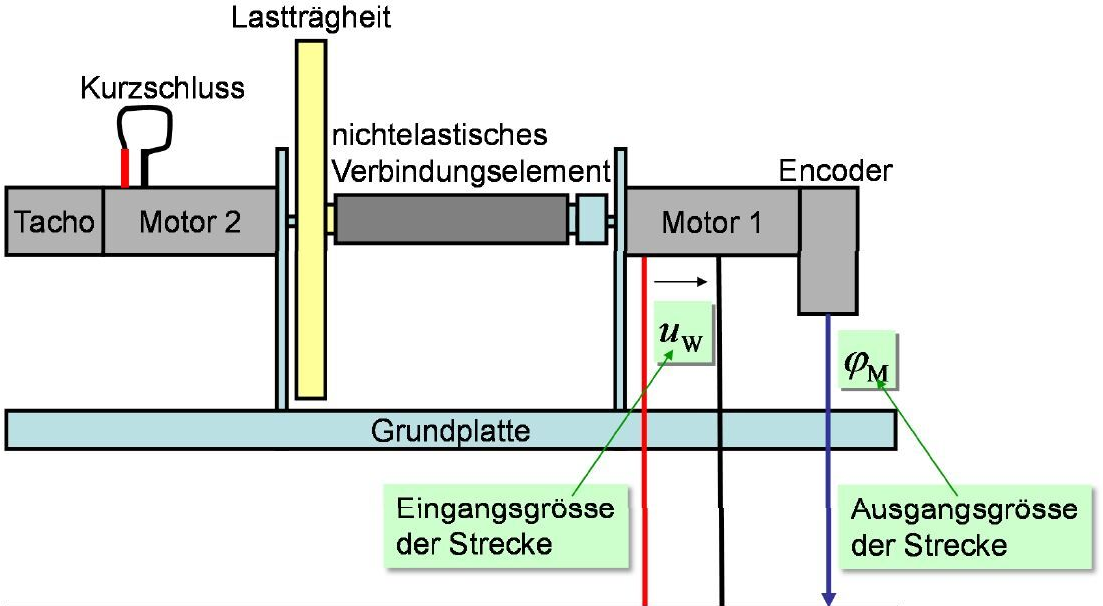
\includegraphics[width=14.5cm]{images/motor_baugruppe.png} %TODO anpassen
	\caption{schematische Darstellung von Motor-Apparatur}
	\label{Ab:motor-baugruppe}
\end{figure}

\section{Motor"=Apparatur}
Die Baugruppe besteht aus einem Motor, Schwungrad und linearen Dämpfer.
Diese drei Komponenten sind miteinander gekoppelt.
Der lineare Dämpfer ist realisiert, durch einen zweiten kurzgeschlossenen Motor.

Die Parameter für das Simulations"=Model konnten grösstenteils aus den Datenblättern der jeweiligen Komponenten entnommen werden. 
Die Dämpfungskonstante des Dämpfers und die Rotationsträgheit der Schwungscheibe mussten berechnet werden.
Die Datenblätter und Berechnungen sind im Repository \textit{\textsc{"}motor\_sim\textit{"}} \footnote{\url{https://github.com/manuelilg/motor\_sim/tree/master/motor\_description/datasheets}} zu finden. 

Für Parameter die nicht im Datenblatt stehen, oder nicht genügend Informationen für eine Berechnung vorhanden waren, wurden geschätzt.
Jedoch haben die geschätzten Parameter in diesem Fallbeispiel keinen nennenswerten Einfluss auf die Simulation.
%Somit haben wir folgende Werte die für die physikalische Beschreibung des Modells.
%Für jeden Link müssen immer die Masse und der Trägheits-tensor definiter sein. Dabei darf die Masse nicht 0 sein und 


\section{Modell}
Für die Apparatur wurde eine Modell"=Beschreibung im \textit{URDF}"=Format erstellt.
Die Kinematische Struktur des Modells ist in der Abbildung \ref{Ab:motor-struktur} dargestellt.
Auffallend ist, dass der Dämpfer noch nicht mit dem Schwungrad gekoppelt ist.
Warum dies so ist, wird im Kapitel \ref{chap:kin-schliessen} erläutert.

\begin{figure}[ht!]
	\centering
\begin{tikzpicture}[scale=1,node distance=10mm,
	link/.style={rectangle, draw=black, thick, inner sep=7},
	joint/.style={ellipse, draw=blue, thick},
	>=latex]
 	
 \node[link] (base) {base\_link};
 \node[joint, above right=of base, xshift=70] (mAxis) {motor\_axis};
 \node[joint, above left=of base, xshift=-70, yshift=-3] (dAxis) {damper\_axis};
 \node[link, above=of mAxis] (motor) {motor};
 \node[link, above=of dAxis] (damper) {damper};
 \node[joint, left=of motor] (coupling) {coupling};
 \node[link, left=of coupling] (flywheel) {flywheel};
 
 \path[->, thick, out=0, in=-130]
 	(base) edge (mAxis);
 \path[->, thick]	
 	(mAxis) edge (motor)
 	(motor) edge (coupling)
 	(coupling) edge (flywheel);
 	
 \path[->, thick, out=180, in=-30]
 	(base) edge (dAxis);
 \path[->, thick]
 	(dAxis) edge (damper);

\end{tikzpicture}
	\caption{kinematische Struktur Motor"=Apparatur}
	\label{Ab:motor-struktur}
\end{figure}

Die komplette Datei ist im Repositiory \textit{\textsc{"}motor\_sim\textit{"}} \footnote{\url{https://github.com/manuelilg/motor_sim/tree/master/motor_description/urdf}} abgelegt.
Ein Ausschnitt aus dieser Datei ist in Auflistung \ref{lst:motor-urdf} gezeigt.

\begin{lstlisting}[language=xml, captionpos=b, caption=Ausschnitt aus motor.urdf, label={lst:motor-urdf}]
<?xml version="1.0"?>
<robot name="motor">

  <link name="world"/>

  <joint name="fixe_base" type="fixed">
    <parent link="world"/>
    <child link="base_link"/>
    <origin xyz="0 0 0.005" rpy="0 0 0"/>
  </joint>

  <link name="base_link">
    <visual>
      <geometry>
        <box size="0.2 0.1 0.01"/>
        <origin xyz="0 0 0.01" rpy="0 0 0"/>
      </geometry>
    </visual>
    <collision>
      <geometry>
        <box size="0.1 0.1 0.01"/>
        <origin xyz="0 0 0.01" rpy="0 0 0"/>
      </geometry>
    </collision>
    <inertial>
      <mass value="1"/>
      <inertia ixx="1" ixy="0.0" ixz="0.0" iyy="1" iyz="0.0" izz="1"/>
    </inertial>
  </link>
...
\end{lstlisting}


%TODO ref auf joint, link

\subsection{Kinematische Kette schliessen}
\label{chap:kin-schliessen}
Das \textit{URDF}"=Format kann keine geschlossenen kinematischen Strukturen abbilden.
Dieser Mangel kann aber behoben werden mit: einem \textit{SDF}"=Joint Eintrag im \textit{URDF} und mit dem \textit{URDF}"=Spezial"=Element \textsc{"}Mimic\textsc{"}.

\subsubsection{SDF"=Joint}
\label{chap:sdf-joint}
Die in diesem Abschnitt erklärte Anpassung wird benötigt, damit in der Simulation das Schwungrad und der Dämpfer miteinander gekoppelt sind.

Im \textit{URDF} können Informationen hinterlegt werden, die nur \textit{Gazebo} interpretiert.
Dafür müssen die Informationen mit dem XML"=Element \textsc{"}gazebo\textsc{"} umschlossen werden.

Wenn man jetzt ein Joint"=Element im \textit{SDF}"=Format einsetzt, kann man die kinematische Struktur schliessen.
Denn die {URDF}"=Datei wird, bevor es ins \textit{Gazebo} geladen wird, ins \textit{SDF}"=Format konvertiert.
Während der Konvertierung werden die Zeilen die sich im XML"=Element \textsc{"}gazebo\textsc{"} befinden einfach ins \textit{SDF} übernommen.

Wie der Eintrag für die Motor"=Baugruppe lauten muss, ist in Auflistung \ref{lst:sdf} gezeigt.
\begin{lstlisting}[language=xml, captionpos=b, caption=SDF-Joint in URDF, label={lst:sdf}]
  <gazebo>
    <joint name="coupling_2" type="fixed">
      <parent>damper</parent>
      <child>flywheel</child>
    </joint>
  </gazebo>
\end{lstlisting}
\subsubsection{Mimic}
\label{chap:mimic}
Der \textit{ROS}"=Knoten \textit{robot\_state\_publisher} berechnet die Transformations"=Daten für die Darstellung der Körper im \textit{RViz}.
Dafür braucht er von allen Gelenken im Modell die Gelenkwinkel.
Das Modell vom \textit{URDF} hat zwei Gelenke, aber das in der Simulation nur eines.
Da in der Simulation die beiden Gelenke fix verbunden sind (siehe Kapitel \ref{chap:sdf-joint}).

Deshalb muss ein Mimic"=Element in einem der beiden Gelenk"=Definitionen eingefügt werden (siehe Auflistung \ref{lst:mimic}). 
\begin{lstlisting}[language=xml, captionpos=b, caption=Mimic in URDF-Joint, label={lst:mimic}, gobble=2]
  <joint name="damper_axis" type="continuous">
    <parent link="base_link"/>
    <child link="damper"/>
    <axis xyz="1 0 0"/>
    <origin xyz="-0.07 0 0.1" rpy="0 0 0"/>
    <dynamics damping="2.1087e-4"/>
    (*\bfseries<mimic joint="motor\_axis\textsc{"} multiplier="1\textsc{"} offset="0"/>*)
  </joint>
\end{lstlisting}

Dieser Eintrag wird vom \textit{ROS}"=Knoten \textit{joint\_state\_publisher}\footnote{\url{http://wiki.ros.org/joint_state_publisher}} interpretiert.
Er bewirkt, dass das Gelenk \textit{\textit{"}damper\_axis\textit{"}} den gleichen Winkel hat, wie das Gelenk \textit{\textit{"}motor\_axis\textit{"}}.
Somit erhalten wir vom \textit{joint\_state\_publisher} für die Eingabe von einem Gelenkwinkel \textit{\textit{"}motor\_axis\textit{"}}, die Ausgabe für die Gelenkwinkel \textit{\textit{"}motor\_axis\textit{"}} und \textit{\textit{"}damper\_axis\textit{"}}.

Diese beiden werden dann vom \textit{robot\_state\_publisher} als Eingabe benötigt.
In Abbildung xx ist der Informationsfluss dargestellt, der aus den oben genannten Fakten resultiert. %TODO ref

\subsection{Gazebo Plugins}
Damit das Modell in der Simulation mit dem \textit{ROS}"=Netzwerk interagieren kann, müssen Plugins eingesetzt werden.

Mit den in Auflistung \ref{lst:plugin} gezeigten Zeilen werden zwei \textit{Gazebo}"=Plugins im Motor"=Modell eingebettet.
\begin{lstlisting}[language=xml, captionpos=b, caption=Plugin in URDF, label={lst:plugin}, gobble=2]
  <gazebo>
    <plugin name="gazebo_ros_joint_force" filename="libgazebo_ros_joint_force.so">
      <robotNamespace>/motor_sim</robotNamespace>
      <topicName>effort</topicName>
      <jointName>motor_axis</jointName>
    </plugin>
  </gazebo>

  <gazebo>
    <plugin name="gazebo_ros_joint_state_publisher" filename="libgazebo_ros_joint_state_publisher.so">
      <robotNamespace>/motor_sim</robotNamespace>
      <jointName>motor_axis</jointName>
      <updateRate>10000.0</updateRate> <!-- to get sure that one every sim step called, up to 10k -->
    </plugin>
  </gazebo>
\end{lstlisting}
%TODO vergleiche kapitel gazebo plugins ??
Das Plugin \textit{\textit{"}gazebo\_ros\_joint\_state\_publisher\textit{"}} misst den Winkel von Gelenk \textit{\textit{"}motor\_axis\textit{"}} und stellt den Messwert zu Verfügung (publish).
Es ist im Standard \textit{ROS"=Package} \textit{\textit{"}gazebo\_ros\_pkgs\textit{"}}~\footnote{\url{http://wiki.ros.org/gazebo_ros_pkgs}} enthalten.
Achtung das Gazebo"=Plugin \textit{\textit{"}gazebo\_ros\_joint\_state\_publisher\textit{"}} ist nicht mit dem ROS"=Knoten \textit{\textit{"}joint\_state\_publisher\textit{"}} zu verwechseln.

Das zweite Plugin \textit{\textit{"}gazebo\_ros\_joint\_force\textit{"}} wird im Abschnitt \ref{chap:joint-force-plugin} genauer erläutert.

\subsubsection{Joint Force Plugin}
\label{chap:joint-force-plugin}
Dieses Plugin wurde im Rahmen dieser Arbeit erstellt und ist im gleichnamigen Repository \textit{\textit{"}gazebo\_ros\_joint\_force\textit{"}}~\footnote{\url{https://github.com/manuelilg/gazebo_ros_joint_force}} zu finden.
Teile von dem Plugin werden vor jedem Simulations"=Schritt aufgerufen und erfüllen somit folgende Aufgaben.
%Das Plugin xx appliziert ein Drehmoment auf das Gelenk xx.
%Die Grösse des Drehmoments erhält das Plugin über das Topic xx.
\begin{itemize}
\item Stellgrösse (Drehmoment) von \textit{EEROS} empfangen
\item Drehmoment auf definiertes Gelenk applizieren
\item Simulation mit \textit{EEROS} synchronisieren
\end{itemize}

\section{Installation}


\section{Ausführen}
\subsection{Gazebo}

\subsection{RViz}
system wird geladen mit robot description
braucht auch tf
%TODO bild info fluss

\section{rqt}
keine speziellen anpassungen an urdf 

\section{Starten}
einzelnen programme gazebo, rviz, rqt


